\documentclass[a4paper,10pt]{report}
\usepackage{fullpage}
\usepackage[utf8]{inputenc}
\usepackage[french]{babel}
\usepackage{amsmath}
\usepackage{geometry}
\geometry{hmargin=1.5cm,vmargin=1.5cm}
\usepackage{xcolor}
\usepackage{graphicx}
\usepackage{graphics}
\usepackage{eurosym} %symbole Euro%
\usepackage{color}

\title{Informatique Répartie - Fédération Bancaire}
\date{2015-2016}
\author{Kafui Atanley \\ Quentin Lerebours \\ Florian Leriche \\ Pauline Mouchès}
\begin{document}
\maketitle
\tableofcontents
\chapter{Introduction}
%	Dans le cadre du projet d'informatique répartie nous allons concevoir une application répartie permettant la gestion d'une fédération bancaire. Ce présent document de conception a pour objectif de définir l'architecture logicielle de notre application.
%En premier lieu voici les fonctionnalités principales de notre applications :
%	\begin{itemize}
%		\item Un système d'authentification permettant au personnel de se connecter sur l'application.
%		\item La création, consultation et édition des comptes clients.
%		\item La gestion des opérations bancaires telles que les virements, les remises de chèque ainsi que les prêts.
%		\item L'envoi de mail aux clients.
%		\item La gestion de statistiques sur l'ensemble des données.
%		\end{itemize}
%En second lieu, cette application sera proposée à plusieurs type d'utilisateur différents. En effet, elle pourra aussi bien être utilisée par les gérants d'une banque que par les employés. Cependant, les gérants auront tous les droits sur cette application alors que les employés seront gérés par ces derniers. Ces utilisateurs n'étant liés qu'à une banque en particulier, nous avons décidé de mettre en place un troisième type d'utilisateur à savoir gérant de la fédération. \\
%	Pour finir, cette application devra pouvoir fonctionner sous windows et Linux et fonctionnera par le biais d'une architecture client/serveur dans laquelle les clients seront les postes et le serveur sera une unique unité centrale par banque.

\chapter{Specifications}


\chapter{Conception préliminaire}

%Cette partie contient de nombreux diagrammes permettant de décrire notre application.
%\section{Diagramme de modèle du domaine}
%\begin{figure}[h!]
%\begin{center}
%   \caption{Diagramme de modèle du domaine}
%   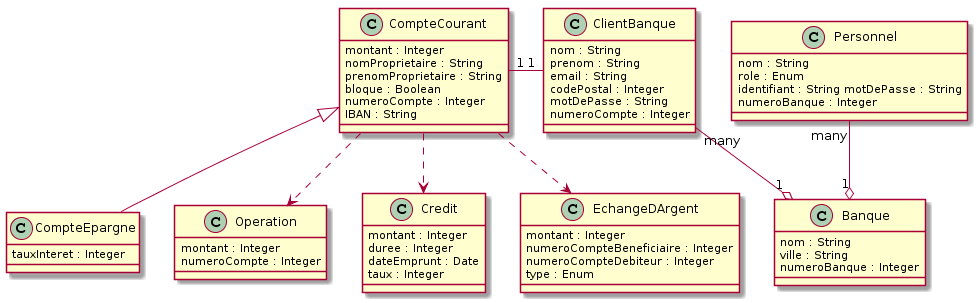
\includegraphics[scale=0.5]{modeleDuDomaine.png}
%   \end{center}
%\end{figure}
%\newpage
%\section{Diagramme d'activité de navigation}
%\begin{figure}[h!]
%\begin{center}
%   \caption{Diagramme de navigation}
%   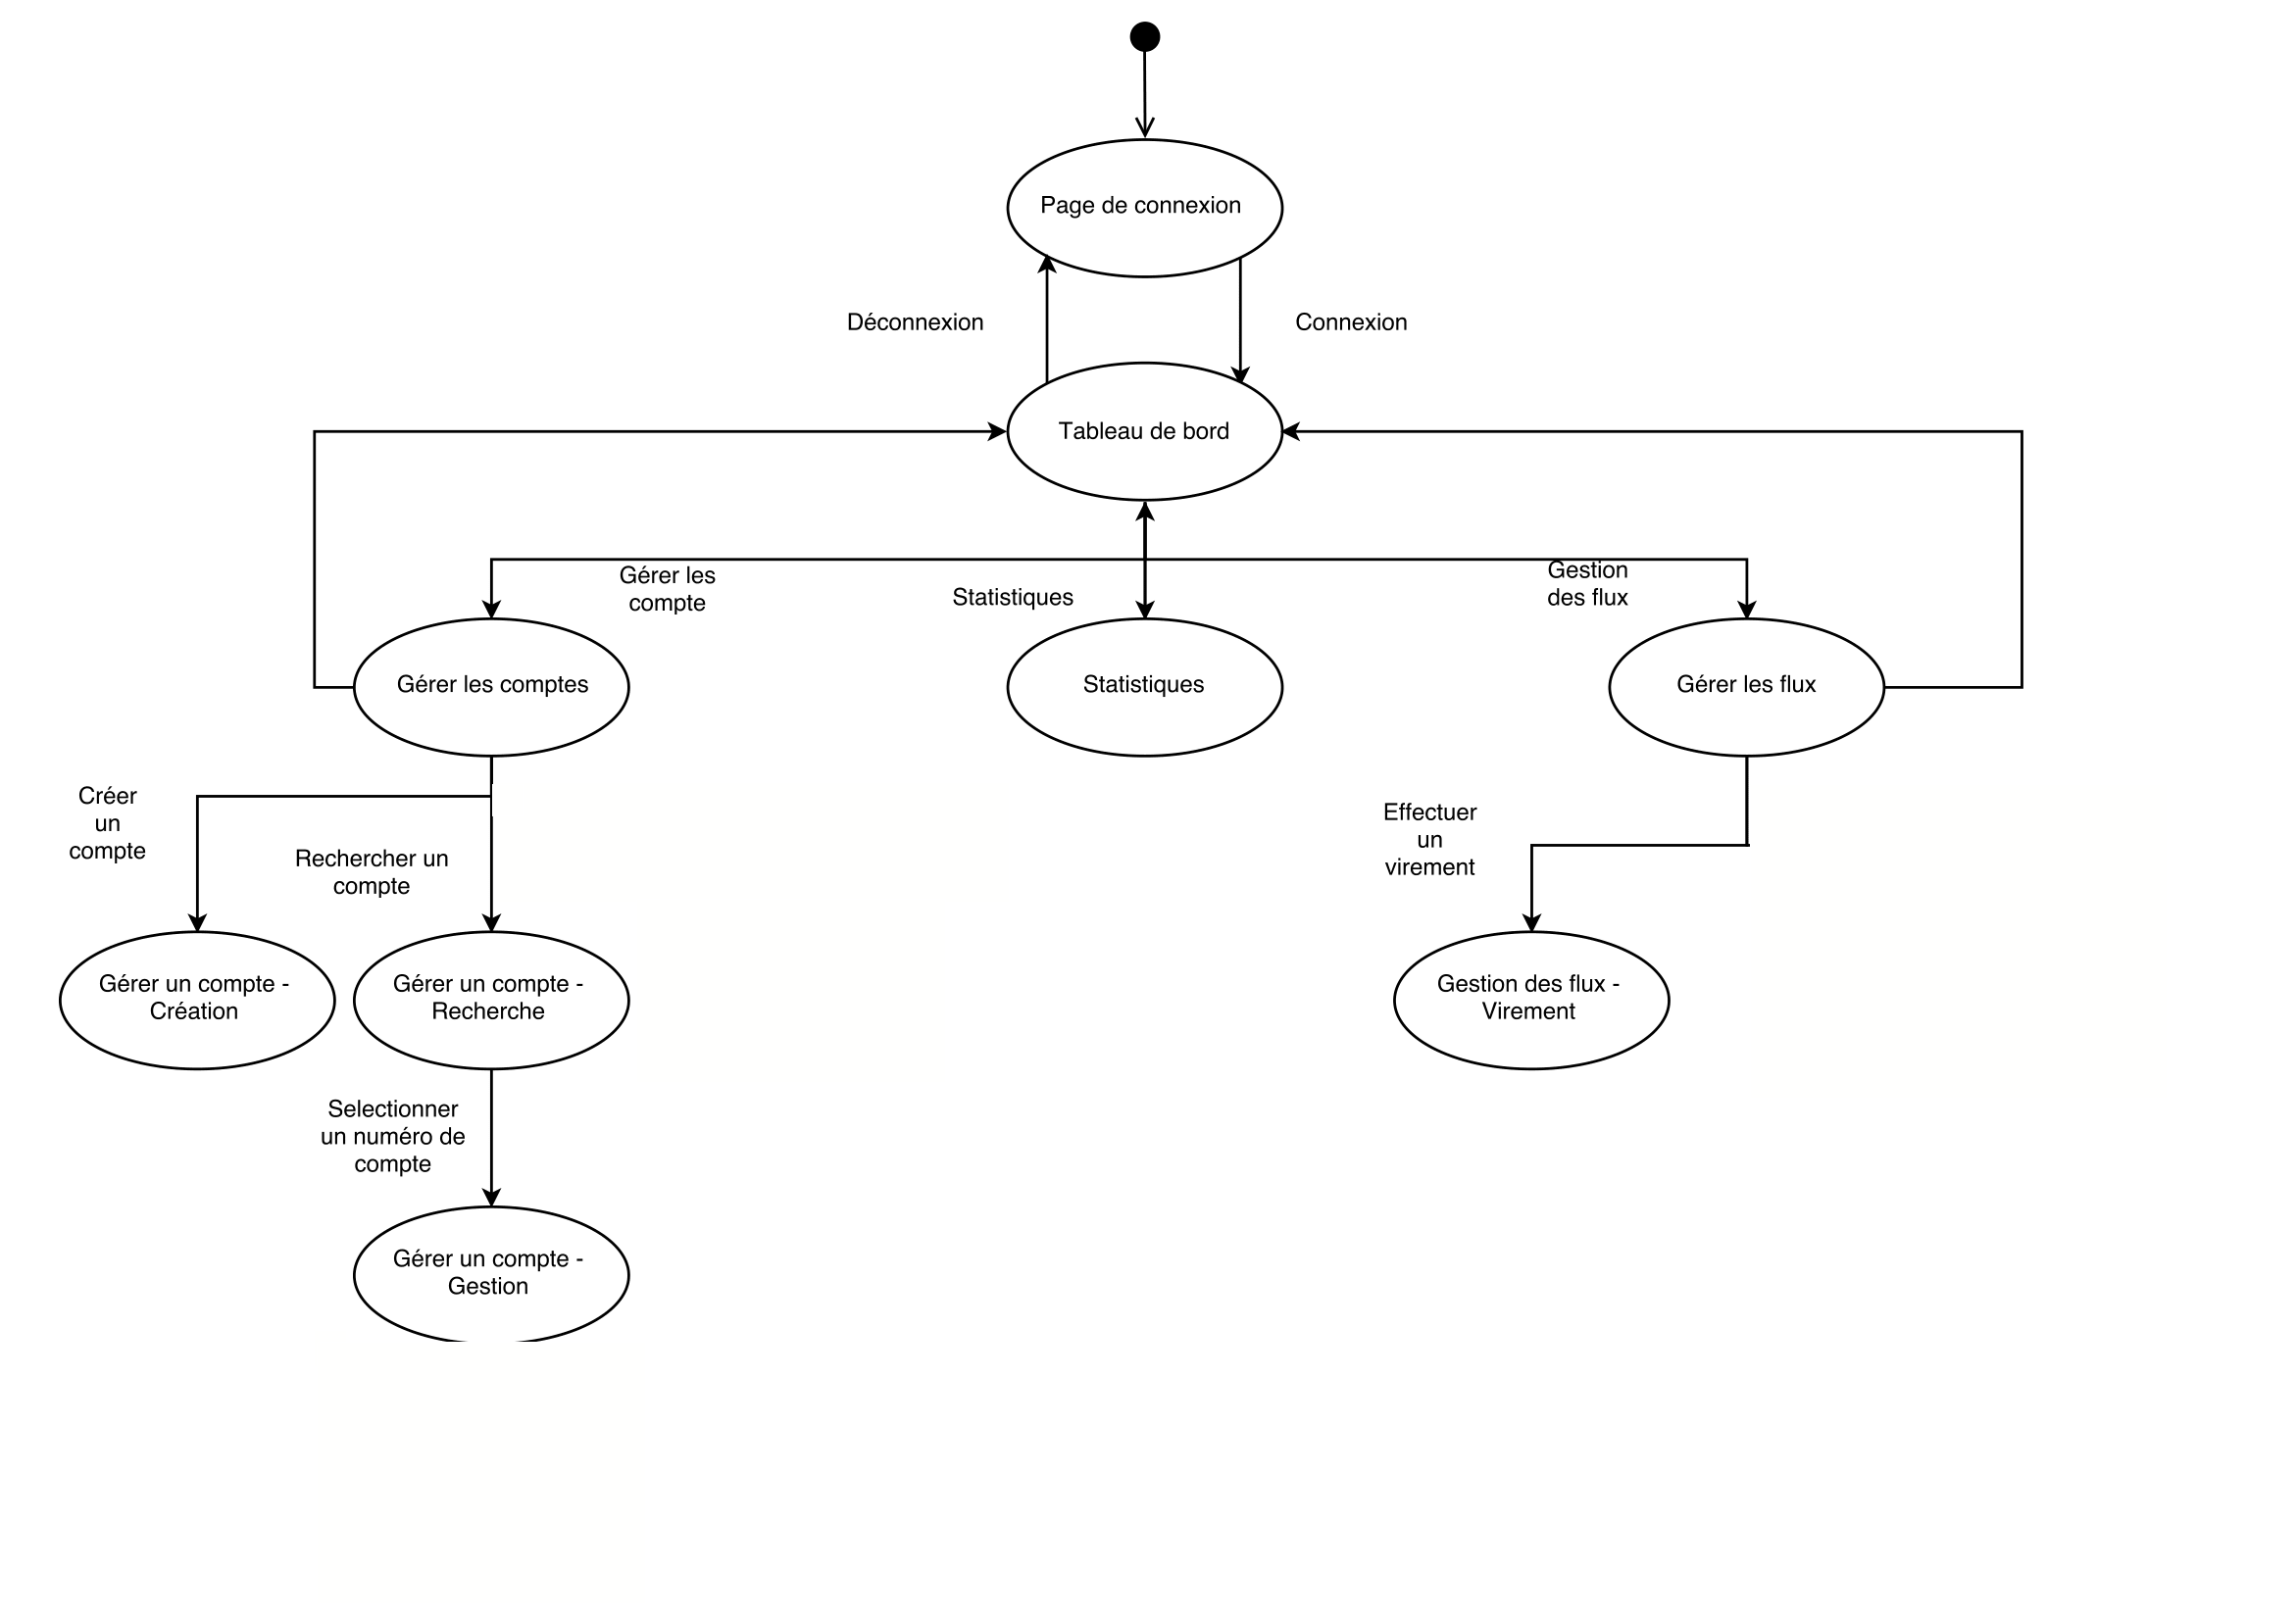
\includegraphics[scale=0.5]{navigation.pdf}
%   \end{center}
%\end{figure}
%\newpage
%\section{Diagrammes d'interaction}
%\subsection{Cas d'utilisation : Se connecter}
%\begin{figure}[h!]
%\begin{center}
%   \caption{Diagramme d'interaction : Se connecter}
%   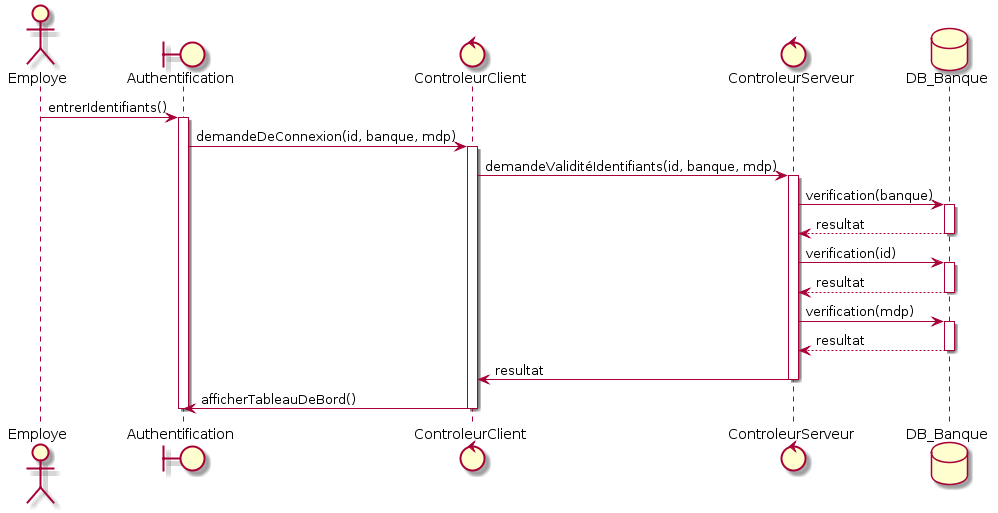
\includegraphics[scale=0.5]{seConnecterIR.png}
%   \end{center}
%\end{figure}
%\subsection{Cas d'utilisation : Créer un compte}
%\begin{figure}[h!]
%\begin{center}
%   \caption{Diagramme d'interaction : Créer un compte}
%   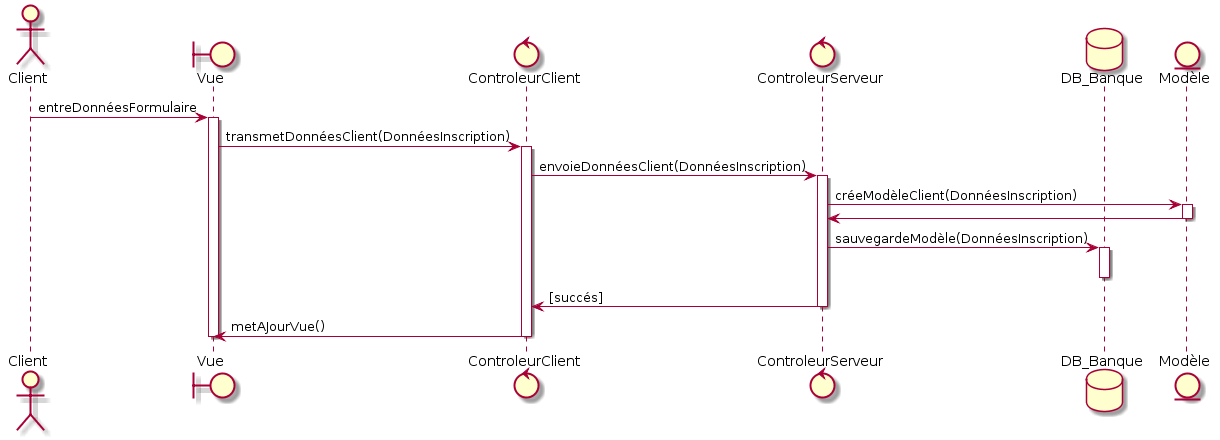
\includegraphics[scale=0.4]{SInscrire.png}
%   \end{center}
%\end{figure}
%\newpage
%\section{Diagramme de classes de conception préliminaire}
%\begin{figure}[h!]
%\begin{center}
%   \caption{Diagramme de classes}
%   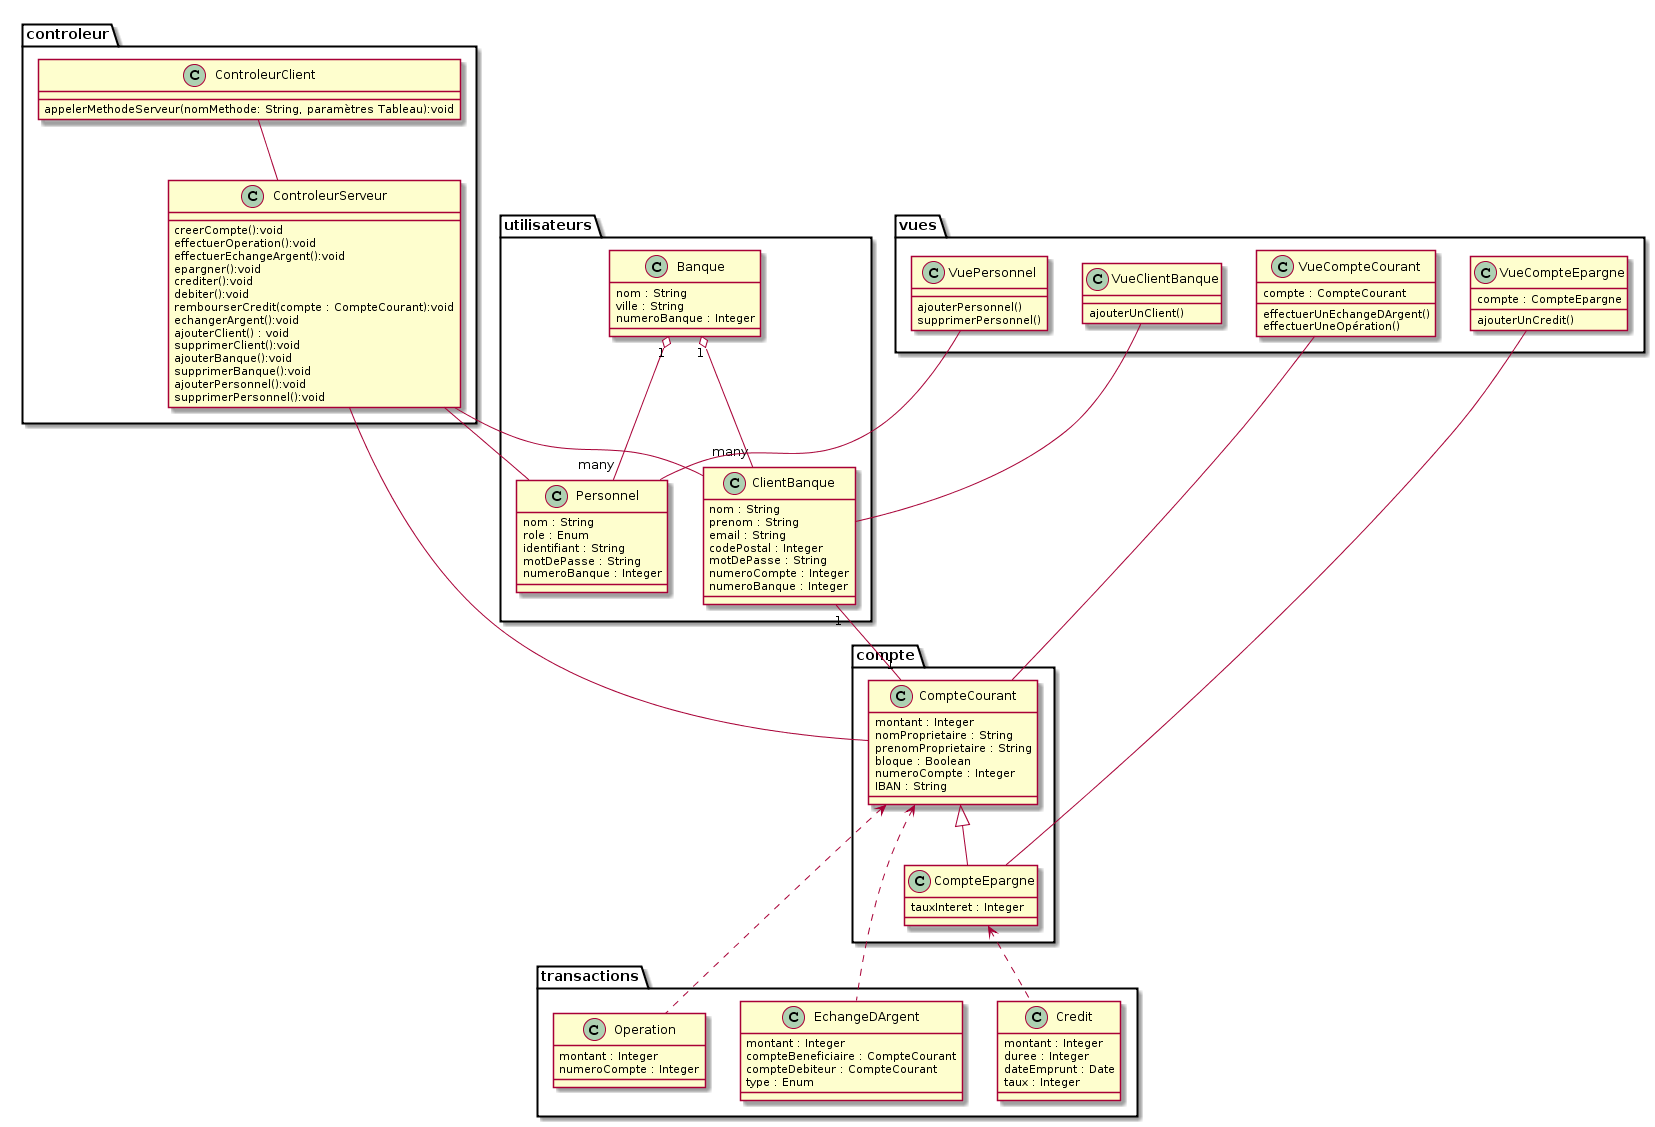
\includegraphics[scale=0.3, angle=90]{diagrammeClasses.png}
%   \end{center}
%\end{figure}
%\newpage


\chapter{Conception détaillée}

%Dans cette partie, chaque package va être décrit. Les attributs et méthodes de chaque classes seront précisées. Le corps des méthodes complexes seront  détaillées grâce à du pseudo-code et commentées.
%
%\section{Package utilisateurs}
%
%\subsection{Banque}
%
%La classe Banque représente une Banque. Une banque possède un nom, une ville et un numéro de banque. L'appartenance à une banque des employés permet de définir leur droits sur les comptes bancaires des clients de la banque.
%
%\subsection{Personnel}
%
%La classe Personnel représente une personne travaillant dans une des banques de la fédération. Un personnel possède un nom, un rôle (employé ou gérant), un identifiant et un mot de passe. En fonction du rôle et du numéro de banque, on peut déduire les droits du personnel.
%
%\subsection{ClientBanque}
%
%La classe ClientBanque représente un client de la banque possédant un compte Bancaire das une des banques de la fédération. Un client de banque possède un nom, un prénom qui permettent d'identifier un et un seul client, un code postal, un mot de passe et un numéro de compte et un numéro de banque.
%
%\section{Package compte}
%
%\subsection{CompteCourant}
%
%La classe CompteCourant représente un compte courant possédé par un client de la banque. Un compte courant possède un montant, un propriétaire  (un nom et un prénom), un booléen bloqué permettant de bloquer le compte par exemple en cas de perte de carte bleue, un numéro de compte, un IBAN permettant d'encaisser des chèques su le compte.
%
%\subsection{CompteEpargne}
%
%La classe CompteEpargne représente un compte épargne possédé par un client de la banque. Cette classe hérite de la classe CompteCourant puisque ces deux classes partagent un grand nombre d'attributs. Un compte épargne possède en plus un taux d’intérêt. Le montant d'un compte épargne augmente chaque année en fonction du taux d’intérêt.  Sur un compte épargne, il est possible d'effectuer un crédit. Ce crédit sera remboursé chaque mois, en fonction du taux du crédit, grâce à l'argent contenu dans le compte.
%
%\section{Package transactions}
%
%\subsection{Operation}
%
%La classe Operation représente un opération qui peut un être : créditer ou débiter le compte. Un transaction possède un montant (positif pour créditer ou négatif pour débiter) et un numéro de compte : le compte sur lequel effectuer la transaction.
%
%\subsection{EchangeDArgent}
%
%La classe EchangeDArgent représente un échange d'argent entre deux comptes via un chèque ou un virement. Un échange d'argent possède un montant, un numéro de compte de bénéficiaire, un numéro de compte de débiteur et un type (chèque ou virement).
%
%\subsection{Credit}
%La classe Credit représente un crédit, c'est à dire un emprunt réalisé à partir d'un compte épargne. Un crédit possède un montant, une durée (durée de remboursement), une date d'emprunt et un taux.
%
%\section{Package vues}
%
%\subsection{VuePersonnel}
%La classe VuePersonnel représente la vue chargée de fournir une représentation graphique des données concernant le personnel de la banque. Elle devra en outre permettre d'informer le contrôleur dans le cas d'un ajout ou d'une suppression d'un membre du personnel.
%\subsection{VueClientBanque}
%La classe VueClientBanque représente la vue chargée de fournir une représentation graphique des données concernant les clients de la banque. Elle devra en outre permettre d'informer le contrôleur dans le cas d'un ajout d'un client dans la banque.
%
%\subsection{VueCompteCourant}
%La classe VueCompteCourant représente la vue chargée de fournir une représentation graphique des données concernant les comptes courants recensés dans la banque. Elle devra en outre permettre d'informer le contrôleur dans le cas où l'utilisateur souhaite effectuer une opération bancaire.
%
%\subsection{VueCompteEpargne}
%La classe VueCompteEpargne représente la vue chargée de fournir une représentation graphique des données concernant les comptes épargnes recensés dans la banque. Elle devra en outre permettre d'informer le contrôleur dans le cas où l'utilisateur souhaite créer un nouveau crédit.
%
%\section{Package controleur}
%
%
%\subsection{ControleurClient}
%Le contrôleur ControleurClient doit permettre de solliciter le contrôleur serveur afin d'appeler les méthodes adéquates. Il devra permettre de récupérer les informations dans le but de les empaqueter en RMI.
%
%\subsection{ControleurServeur}
%Le contrôleur ControleurServeur permet d'interpréter les actions de l'utilisateur et d'appeler les méthodes du modèle dans le but de le mettre à jour. Il permet la gestion des ressources humaines de la banque, des diverses opérations bancaires ainsi que des comptes bancaires.
%détail des méthodes

\chapter{Implémentation et tests}


\chapter{Conclusion et perspectives}

\end{document}\grid
\grid
